\documentclass[
    reprint, 
    aps,
    preprintnumbers,
    twocolumn,
    prb,
    superscriptaddress
]{revtex4-2}


%=======================
% Packages:
%=======================

\usepackage[utf8]{inputenc}
\usepackage{booktabs}
\usepackage[multiple]{footmisc}
\usepackage{lipsum}
\usepackage{rotating}
\usepackage{perpage}
\usepackage{chronology}
\usepackage{lipsum}
\usepackage{amssymb}
\usepackage{amsbsy}
\usepackage{amsmath}
\usepackage{tikz}
\usepackage[T1]{fontenc}
\usepackage{etoolbox}
\usepackage{graphics}
\usepackage{abraces}
\makeatletter
\let\unit\relax % otherwise there are package conflicts with siunitx
\makeatother
\usepackage{siunitx}
\usepackage{hyperref}
%\usepackage{float}
\usepackage{multirow}
\usepackage{mathtools}
\usepackage{bm}
\usepackage{url}
\usepackage{physics}
\usepackage{hyperref}
\usepackage{bbm}
\usepackage{color}
\usepackage{placeins}
\usepackage[normalem]{ulem}
\usepackage{mhchem}

%=======================
% New Commands:
%=======================

\newcommand{\vk}{\vec{k}}
\newcommand{\vQ}{\vec{Q}}
\newcommand{\up}{\uparrow}
\newcommand{\down}{\downarrow}
\newcommand{\kplusQ}{\vk+\vQ}
\newcommand{\kminusQ}{-\vk-\vQ}

\newcommand{\ddt}{\frac{\mathrm{d}}{\mathrm{d}t}}
\newcommand{\dgamma}{\mathrm{d}\gamma}

\newcommand{\mM}{\mathcal{M}}
\newcommand{\mN}{\mathcal{N}}

\begin{document} 

% Preliminary title
\title{Collective excitations in competing phases in two and three dimensions}

%=======================
% Authors:
%=======================

\author{Joshua Alth\"user}\email{joshua.althueser@tu-dortmund.de}
\affiliation{Condensed Matter Theory, TU Dortmund University,
Otto-Hahn Stra\ss{}e 4, 44221 Dortmund, Germany}

\author{G\"otz S.~Uhrig}
\email{goetz.uhrig@tu-dortmund.de}
\affiliation{Condensed Matter Theory, TU Dortmund University,
Otto-Hahn Stra\ss{}e 4, 44221 Dortmund, Germany}

\date{\today}

%%%%%%%%%%%%%%%%%%%%%%%%%%%%%%%%%%%%%%%%%%%%%%%%%%%%%%%%%%%%%%%%%%%%%%%%%%%%%%%%%%%%%%%%%%%%%%%%%%%%%%%%%%%%%%%%%%%%%
%%%%%%%%%%%%%%%%%%%%%%%%%%%%%%%%%%%%%%%%%%%%%%%%%%%%%%%%%%%%%%%%%%%%%%%%%%%%%%%%%%%%%%%%%%%%%%%%%%%%%%%%%%%%%%%%%%%%%
%%%%%                                                  Abstract                                                 %%%%%
%%%%%%%%%%%%%%%%%%%%%%%%%%%%%%%%%%%%%%%%%%%%%%%%%%%%%%%%%%%%%%%%%%%%%%%%%%%%%%%%%%%%%%%%%%%%%%%%%%%%%%%%%%%%%%%%%%%%%
%%%%%%%%%%%%%%%%%%%%%%%%%%%%%%%%%%%%%%%%%%%%%%%%%%%%%%%%%%%%%%%%%%%%%%%%%%%%%%%%%%%%%%%%%%%%%%%%%%%%%%%%%%%%%%%%%%%%%
\begin{abstract}
    We investigate the superconducting (SC), charge-density wave (CDW), and antiferromagnetic (AFM) phases 
    in the extended Hubbard model at zero temperature and half-filling.
    We employ the iterated equations of motion approach \cite{Kalthoff17,bleicker18} to compute the two-particle Green's functions and by extension, the corresponding spectral densities.
    This renders comprehensive analysis of the behaviour of collective excitations possible as the model's parameters are changed across phase transitions.
    We identify the well-known amplitude (Higgs) and phase (Leggett) modes within the superconducting phase and observe a similar excitation in the CDW phase which shifts towards zero energy as the system approaches the phase transition to the SC phase.
    In the CDW phase, close to the phase transition to the AFM phase, we find a collective mode that does not change significantly and another mode that becomes soft as the phase boundary is approached.
\end{abstract}

\maketitle

%%%%%%%%%%%%%%%%%%%%%%%%%%%%%%%%%%%%%%%%%%%%%%%%%%%%%%%%%%%%%%%%%%%%%%%%%%%%%%%%%%%%%%%%%%%%%%%%%%%%%%%%%%%%%%%%%%%%%
%%%%%%%%%%%%%%%%%%%%%%%%%%%%%%%%%%%%%%%%%%%%%%%%%%%%%%%%%%%%%%%%%%%%%%%%%%%%%%%%%%%%%%%%%%%%%%%%%%%%%%%%%%%%%%%%%%%%%
%%%%%                                                Introduction                                               %%%%%
%%%%%%%%%%%%%%%%%%%%%%%%%%%%%%%%%%%%%%%%%%%%%%%%%%%%%%%%%%%%%%%%%%%%%%%%%%%%%%%%%%%%%%%%%%%%%%%%%%%%%%%%%%%%%%%%%%%%%
%%%%%%%%%%%%%%%%%%%%%%%%%%%%%%%%%%%%%%%%%%%%%%%%%%%%%%%%%%%%%%%%%%%%%%%%%%%%%%%%%%%%%%%%%%%%%%%%%%%%%%%%%%%%%%%%%%%%%

\section{Introduction}\label{sec:introduction}

The Hubbard model has been studied in a plethora of previous studies. 
Early studies proved the existence of eigenstates to the Hubbard Hamiltonian that exhibit off-diagonal long-range order,
encouraging the model's usage for the description of high-temperature superconductivity \cite{yang89}.
Shortly afterward, an exact SO(4) symmetry was discovered,
which allows a degeneracy of superconductivity (SC) and a charge-density wave (CDW) governed by an attractive on-site interaction \cite{yang90}.
This coexistence can be argued by the existence of a particle-hole transformation on bipartite lattices, 
that maps the attractive Hubbard model exactly onto the repulsive one, exhibiting antiferromagnetism (AFM) \cite{Hirsch85}.
The previously mentioned SC and CDW phases map to different spin operators \cite{zitko15,lieb89}.

Many recent experimental and theoretical studies examined the driven systems in the hope of inducing superconductivity 
\cite{Nicoletti14,Krull14,Moor14,Casandruc15,patel16,sentef17,Buenemann17}.
Other studies, focusing on equilibrium systems, 
investigated the phases and various quantities therein of the said model including various additional interactions with and without doping 
\cite{Micnas88,Micnas88b,Micnas89,Dzierzawa92,Kostyrko92,Eriksson95,Staudt00,Onari04,Toschi05,Brackett16,Paki19,romer20,Sushchyev22}.

In this paper, we will restrict ourselves to the half-filled Hubbard model, including an additional intersite interaction, on a square and a simple cubic lattice.
\textcolor{red}{Für den 3D Fall finde ich keine Phasendiagramme des extended Hubbard models, ggf nochmal suchen...}
The 2D case already exhibits a wide range of possible phases, including CDW, AFM as well as $s$- and $d_{x^2 - y^2}$-wave superconductivity
\cite{Micnas88b,Tsuchiura95,Su01,Su04,ha11,Huang13,Jiang22}.

In this article, we will first employ a mean-field approximation to the interaction terms 
and then use the methodology from the so-called iterated equations of motion approach (iEoM),
which has already seen success in the handling of interaction quenches \cite{uhrig09,hamerla13,hamerla14,bleicker18}.
Here, one commutes operators from a suitable operator basis with the Hamiltonian and adds the newly occurring terms to it.
Naturally, a truncation is necessary for most practical applications, however, the approximation becomes better the more terms are included within the basis.
The functionality of this method has been compared to the density matrix formalism and has proved to be considerably more accurate \cite{Kalthoff17}.
Additionally, we will show an explicit way to obtain various Green's functions from the aforementioned methodology.
By extension, we also obtain the spectral functions of the investigated systems and discuss the excitations found therein.
The prominent examples in the SC phase are the well-known phase (Leggett) and amplitude (Higgs) modes \cite{Cea14,Krull16,Schwarz20,Fan22}.

The remainder of this paper is organized as follows:
In \autoref{sec:model} we will introduce the model and its Hamiltonian as well as our mean-field theory.
A brief overview of the iterated equations of motion approach is presented in \autoref{sec:ieom}.
Next, we show our results in \autoref{sec:results}.
Lastly, in \autoref{sec:conclusion}, we will discuss our results.
In the appendix \textcolor{red}{(or in the supplemental material?)}, we will derive and explain our methods in detail.

\section{Model and mean-field theory}\label{sec:model}

\subsection{Model}

\textcolor{red}{Schreiben wie cool das Hubbard Model ist}

The Hamiltonian of the extended Hubbard model is given by
\begin{equation}
    \label{eqn:full_hamiltonian}
    \begin{aligned}
        H = &-t \sum_{\langle i, j \rangle, \sigma} \left( c_{i\sigma}^\dagger c_{j\sigma} + \text{h.c.} \right) 
        + \mu \sum_{i,\sigma} n_{i\sigma} \\
        &+ U \sum_{i} n_{i\uparrow} n_{i\downarrow} 
        + \frac{V}{2} \sum_{\langle i, j\rangle, \sigma} n_{i\sigma} n_{j\sigma}\,,
    \end{aligned}
\end{equation}
where $c_{i\sigma}^{(\dagger)}$ annihilates (creates) an electron with spin $\sigma$ on lattice site $i$ 
and $\langle i, j\rangle$ denotes the summation over next neighbours.
The parameters are the hopping amplitude $t$, the onsite interaction $U$, the intersite interaction $V$, and the chemical potential $\mu$.
Applying a Fourier-transformation into $k$-space yields the single-particle dispersion 
\begin{equation}
    \epsilon_0 (\vk) = -2t \sum_{\alpha=1}^D \cos(k_\alpha)\,,\quad k_\alpha \in [-\pi, \pi)\,,
\end{equation}
with the system's dimension $D$ and the dimensionless momentum $\vk$.

\subsection{Static mean-field theory}

Next, we decouple the interaction terms.
We define 
\begin{equation}
    \label{eqn:operators}
    \begin{aligned}
        n_{k\sigma} &\coloneqq  c_{\vk\sigma}^\dagger c_{\vk\sigma}\,,      &f_k     &\coloneqq  c_{-\vk\down} c_{\vk\up}\,, \\
        g_{k\sigma} &\coloneqq  c_{\vk\sigma}^\dagger c_{\vk+\vQ\sigma}\,,  &\eta_k  &\coloneqq  c_{-\vk-\vQ\down} c_{\vk\up}\,,
    \end{aligned}
\end{equation}
where $\vQ \coloneqq  (\pi, ...)$ defines the nesting vector for the CDW and AFM phases, see Ref. \cite{sentef17}.
We use the following abbreviations to write down the mean-field parameters
\begin{subequations}
    \begin{align}
        \label{eqn:delta_cdw}
        \Delta_\text{CDW} &= \left(\frac{U}{2N} - \frac{zV}{N}\right) \sum_{\vk\sigma} \langle g_{\vk\sigma} \rangle\,, \\
        \label{eqn:delta_afm}
        \Delta_\text{AFM} &= \frac{U}{2N} \sum_{\vk} \left( \langle g_{k\uparrow} \rangle - \langle g_{\vk\downarrow} \rangle \right)\,, \\
        \Delta_\text{SC} &= \frac{U}{N} \sum_{\vk} \langle f_{\vk} \rangle\,, \\
        \Delta_\eta &= \frac{U}{N} \sum_{\vk} \langle \eta_{\vk} \rangle\,, \\
        \Delta_n &= \frac{V}{N} \sum_{\vk,\sigma} \sum_{\alpha=1}^D \cos k_\alpha \langle n_{\vk\sigma} \rangle\,,
    \end{align}
\end{subequations}
where $z$ denotes the coordination number of the lattice.
The last parameter, $\Delta_n$, renormalizes the hopping term to
\begin{equation}
    \epsilon( \vk ) \coloneqq  -(2 + \Delta_n) \sum_{\alpha=1}^D \cos(k_\alpha)\,.
\end{equation}
In total, we obtain the mean-field Hamiltonian in spinor representation as
\begin{equation}
    \label{eqn:mf_hamiltonian}
    H_\text{MF} = \sum_{\vk} \Psi^\dagger (\vk) h(\vk) \Psi (\vk)\,,
\end{equation}
with the spinors
\begin{equation}
    \Psi^\dagger (\vk) \coloneqq  \left( c_{\vk\up}^\dagger\,, c_{\kplusQ\up}^\dagger\,, c_{-\vk\down}\,, c_{\kminusQ\down} \right)
\end{equation}
and 
\begin{equation}
    h(\vk) \coloneqq  \begin{pmatrix}
        \epsilon (\vk) & \Delta_-^* & \Delta_\text{SC} & \Delta_\eta \\
        \Delta_- & \epsilon (\vk + \vQ) & \Delta_\eta & \Delta_\text{SC} \\
        \Delta_\text{SC}^* & \Delta_\eta^* & - \epsilon (-\vk) & - \Delta_+ \\
        \Delta_\eta^* & \Delta_\text{SC}^* & - \Delta_+^* & - \epsilon (-\vk - \vQ)
        \end{pmatrix}\,,
\end{equation}
where we defined $\Delta_\pm \coloneqq \Delta_\text{CDW} \pm \Delta_\text{AFM}$.

\begin{figure}
    \centering
    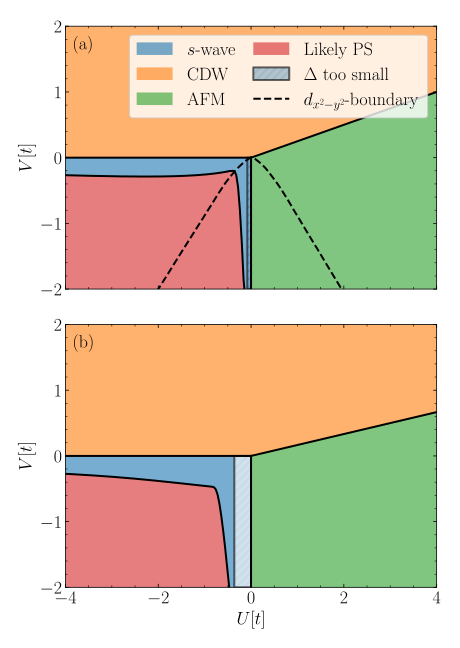
\includegraphics[width=.48\textwidth]{plots/phase_diagram.pdf}
    \caption{The phase diagram obtained for the extended Hubbard model on 
    (a) a square lattice and (b) a simple cubic lattice using a mean-field approximation at temperature $T=0$.
    The CDW-AFM boundary lies at $U = zV$, where $z$ is the coordination number. 
    For $U<0$ and $V=0$, there is a coexistence of CDW and $s$-wave SC.
    The boundary for the $d_{x^2 - y^2}$-wave SC (dashed line) for the square lattice has been taken from Ref. \cite{Micnas88b}, 
    as it is not accessible using our formalism.}
    \label{fig:phase_diagram}
\end{figure}

We observe that the entire Hamiltonian and thus all expectation values only depend on
\begin{equation}
    \hat{\gamma}(\vk) \coloneqq \frac{1}{D} \sum_{\alpha=1}^D \cos(k_\alpha)\,,
\end{equation}
i.e., for any operator $\hat{O}$ the following relation holds 
\begin{equation}
    \label{eqn:equal_expecs}
    \langle \hat{O}_{\vk} \rangle = \langle \hat{O}_{\vk'} \rangle \eqqcolon \langle \hat{O}( \gamma ) \rangle\,,
\end{equation}
if $\hat{\gamma}(\vk) = \hat{\gamma}(\vk')$.
While two-dimensional systems around the size of $100\times100$ lattice sites can still be solved by using momentum sums,
computing solutions for large three-dimensional systems becomes impossible due to the $N=L^3$ scaling.
This issue can be resolved by using the aforementioned fact and replacing the momentum sums with energy integrals using the bare density of states (DOS)
\begin{equation}
    \rho(\gamma) \coloneqq  \frac{1}{N} \sum_{\vk} \delta \left(\gamma - \hat{\gamma} (\vk) \right)\,.
\end{equation}
As an example, we consider 
\begin{equation}
    \Delta_\text{SC} = \frac{U}{2N} \int_{-1}^{1} \dgamma \rho(\gamma) \langle f( \gamma ) \rangle\,.
\end{equation}
We will be using the exact densities of states for the square and the simple cubic lattice found in Ref. \cite{Hanisch97}.
This allows us to access both two- and three-dimensional models on equal footing.
We can compute any phase as long as it does not introduce another kind of momentum dependence.

We solve the mean-field equations self-consistently.
The $\gamma$-integrals are approximated numerically using a $\tanh$-$\sinh$ quadrature \cite{takahasi73}, 
terminating once $|1 - \int \dgamma \rho(\gamma)| < 10^{-13}$ and reusing the computed points and weights.
This method excels at dealing with the singularities in the DOS, 
requiring merely a few hundred function evaluations to achieve the desired accuracy.

This procedure yields the ground state phase diagram at temperature $T=0$ shown in \autoref{fig:phase_diagram}.
The CDW-AFM boundary is located at $U = zV$, where $z$ is the coordination.
This holds for both the square lattice ($z=4$) and the simple cubic lattice ($z=6$) and can be seen by comparing \eqref{eqn:delta_cdw} and \eqref{eqn:delta_afm}:
Crossing the aforementioned line, changes which one of the two prefactors is larger.

Note, that the $d_{x^2 - y^2}$-superconducting state, which has been confirmed for the square lattice \cite{Micnas88b,Huang13}, cannot be described by our method. 
This is due to our restriction to terms that are proportional to $\hat{\gamma}(\vk)$.

%%%%%%%%%%%%%%%%%%%%%%%%%%%%%%%%%%%%%%%%%%%%%%%%%%%%%%%%%%%%%%%%%%%%%%%%%%%%%%%%%%%%%%%%%%%%%%%%%%%%%%%%%%%%%%%%%%%%%
%%%%%%%%%%%%%%%%%%%%%%%%%%%%%%%%%%%%%%%%%%%%%%%%%%%%%%%%%%%%%%%%%%%%%%%%%%%%%%%%%%%%%%%%%%%%%%%%%%%%%%%%%%%%%%%%%%%%%
%%%%%                                                  Methods                                                  %%%%%
%%%%%%%%%%%%%%%%%%%%%%%%%%%%%%%%%%%%%%%%%%%%%%%%%%%%%%%%%%%%%%%%%%%%%%%%%%%%%%%%%%%%%%%%%%%%%%%%%%%%%%%%%%%%%%%%%%%%%
%%%%%%%%%%%%%%%%%%%%%%%%%%%%%%%%%%%%%%%%%%%%%%%%%%%%%%%%%%%%%%%%%%%%%%%%%%%%%%%%%%%%%%%%%%%%%%%%%%%%%%%%%%%%%%%%%%%%%

\section{Iterated equations of motion and Green's functions}\label{sec:ieom}

So far we have discussed the static mean-field equations that essentially describe the static ground state.
These results will be used to compute the quantities, namely expectation values, necessary for the iterated equations of motion approach \cite{uhrig09,hamerla13,hamerla14,bleicker18}.
With it, we can describe two-particle quantities like the various collective excitations of the system.
We will present the general ideas briefly here and refer the interested reader to the appendix \textcolor{red}{!REF!} for a detailed explanation and derivation.

We start with some operator set $\mathcal{B}$ that is complete with respect to commutation with a Hamiltonian $H$, 
i.e., any commutator $[H, A]$ for any $A \in \mathcal{B}$ can be represented by linear combinations of operators in $\mathcal{B}$.
We can then express any time-dependent operator from this set as
\begin{equation}
    a(t) = \sum_j c_j(t) A_j\,,
\end{equation}
where $c_j(t)$ captures the entire time dependence. 
Inserting this into the Heisenberg equation of motion and applying an operator scalar product $(A_i|\cdot)$ to both sides of the equation yields
\begin{equation}
    \label{eqn:heisenberg}
    \begin{aligned}
        \ddt a(t) = \sum_j \ddt c_j(t) A_j &= i \sum_j c_j(t) [H, A_j] \\
        \Rightarrow \sum_j \underbrace{(A_i | A_j)}_{\coloneqq \mN_{ij}} \ddt c_j(t) &= i \sum_j \underbrace{(A_i | [H, A_j])}_{\coloneqq \mM_{ij}} c_j(t) \\
        \Rightarrow \mN \ddt \vec{c}(t) &= i \mM \vec{c}(t)\,.
    \end{aligned}
\end{equation}
The matrices $\mN$ and $\mM$ contain all the dynamics and energetic properties of the system.
The advantage is that one can now handle simple matrices rather than operators acting on an enormous Hilbert space.
The size of these matrices depends entirely on the set of operators.

However, most Hamiltonians do not allow any such operator set to exist as the commutation usually introduces terms of higher order.
For instance, commuting a bilinear term with a quartic Hamiltonian yields, quartic terms. Repeating the commutation yields hexartic ones and so on.
Therefore, one repeats this commutation process and includes the occurring terms within a bigger set,
hoping to get better results as the set size increases.

In this article, we will be using the operator pseudo scalar product
\begin{equation}
\label{eqn:scalar_product}
    (A | B) \coloneqq  \langle [A^\dagger, B] \rangle\,,
\end{equation}
where the expectation values are taken with respect to the thermal equilibrium of the mean-field Hamiltonian \eqref{eqn:mf_hamiltonian}.
Note, that this is not a proper scalar product, as a norm defined using it can also be negative.
For example, assume that for some operator $A$
\begin{equation}
    ||A|| = (A | A) = \langle [A^\dagger, A] \rangle > 0\,,
\end{equation}
then
\begin{equation}
    ||A^\dagger|| = (A^\dagger | A^\dagger) = \langle [A, A^\dagger] \rangle = - ||A|| < 0\,.
\end{equation}
We will compute $\mM$ by commutating with the full Hubbard Hamiltonian \eqref{eqn:full_hamiltonian} enabling us to capture collective behaviour rather than the one particle dynamics given by the mean-field approximation.

We create our operator set on the basis of \eqref{eqn:equal_expecs}.
It consists of operators of the type
\begin{equation}
    A_\gamma \coloneqq \frac{1}{\sqrt{N}} \sum_{\vk} \delta (\gamma - \hat{\gamma}( \vk )) A_{\vk}\,,
\end{equation}
where $A_{\vk}$ represents each type of operator in \eqref{eqn:operators} and their Hermitian conjugates.
Operators with different indices are put into the set individually, e.g., $n_{\gamma \up}$, and $n_{\gamma \down}$ are distinct operators in our set.

Naturally, we have to discretize $\gamma$, 
however, this allows us to obtain good results with drastically smaller matrices compared to a momentum-based operator set and obtain results for a three-dimensional system in the first place.
Practically, we choose $N_\gamma = 3000$ equally spaced discretization points.
A detailed explanation of the numerics is provided in the appendix \textcolor{red}{!REF!}.

Next, we order these operators in a way reminiscent of the $x$- and $p$-terms in the harmonic oscillator, i.e.,
\begin{equation}
    X_i \coloneqq  A_i + A_i^\dagger\,,\quad P_i \coloneqq  A_i - A_i^\dagger\,.
\end{equation}
Then, our set is given by $\mathcal{B}_{XP} \coloneqq \{ X_i, P_i \}$.
If some operators would be 0 ($P_i$ for any $n$-type term) or duplicates (certain $X_i$ for $g$-type terms), we omit them.

Due to this choice of set, the matrices occurring in \eqref{eqn:heisenberg} have a special block structure
\begin{equation}
    \label{eqn:xp_set}
    \mM = \begin{pmatrix}
        \mathcal{K}_+ & \kappa \\ \kappa^\dagger & \mathcal{K}_-
    \end{pmatrix}\,,\quad \mN = \begin{pmatrix}
        \Lambda_+ & \mathcal{L} \\ \mathcal{L}^\dagger & \Lambda_-
    \end{pmatrix}\,,
\end{equation}
where the upper block refers to all $X_i$ and the lower block to all $P_i$.
Furthermore, due to symmetry, the relations $\Im [\mathcal{K}_\pm] = \Re [\kappa] = 0$ and $\Re [\Lambda_\pm] = \Im [\mathcal{L}] = 0$ hold.
Thus, if all occurring expectation values are real, both matrices have large empty blocks.
This condition is fulfilled for all cases investigated in this article.
Additionally, the matrix $\mM$ is positive semidefinite if the system is in thermal equilibrium.
We proof this statement in the appendix \textcolor{red}{!REF!}.

To study the collective excitations, we investigate various retarded Green's functions 
\begin{equation}
    G_{AB}^\text{ret} (t) = - i \langle [A(t), B] \rangle \Theta(t)\,,
\end{equation}
and their Fourier-transformed
\begin{equation}
    \label{eqn:standard_gf}
    G_{AB}(\omega + i0^+) = -i \int_0^{\infty} e^{izt} \langle [A(t), B] \rangle \mathrm{d}t\,,
\end{equation}
where $\Theta(t)$ is the Heaviside function.
Our previous choice of pseudo scalar product enables us to write down a matrix-valued Green's functions in terms of the aforementioned matrices
\begin{align}
    \label{eqn:green_function}
    \mathcal{G}(z &= \omega + i0^+) = \mN \frac{1}{-z \mN - \mM} \mN \\
        &\coloneqq  -\mN \mathcal{R}(z) \mN\,,
\end{align}
where we used the resolvent
\begin{equation}
    \label{eqn:resolvent}
    \mathcal{R}(z) \coloneqq  \frac{1}{z \mN + \mM}\,.
\end{equation}
The entries of this matrix $\mathcal{G}(z)$ are the Fourier-transformed Green's functions mentioned in \eqref{eqn:standard_gf} with respect to the operators from the initially chosen set.
For instance, assume the operator in the set is $f_{\vk}$, then the top left element of $\mathcal{G}$ is the Green's function 
\begin{align}
    \mathcal{G}_{00}(z = \omega +i0^+) &=  G_{f_{\vk}(t) f_{\vk}^\dagger} (z) \nonumber \\
        &= -i \int_0^{\infty} \langle [f_{\vk}(t), f_{\vk}^\dagger(0)] \rangle e^{izt} \mathrm{d}t\,.
\end{align}

In the following, we will derive this relation.
For that, consider the Fourier-transformed Green's function \eqref{eqn:standard_gf} with respect to two operators $A$ and $B^\dagger$ that are included in our operator set
\begin{align}
    G_{AB^\dagger} (z) &= - i \int_0^\infty \exp(izt) \langle [ A(t), B^\dagger(0) ] \rangle \mathrm{d}t
\end{align}
Since $A$ and $B$ are included in the operator set, we can rewrite them as dot products of the vector
\begin{equation}
    \vec{A} \coloneqq  \left( A_1, A_2, \dots, A_N \right)\,, \quad
    \vec{A}^\dagger \coloneqq  \begin{pmatrix}
        A_1^\dagger \\ A_2^\dagger \\ \vdots \\ A_N^\dagger
    \end{pmatrix}\,,
\end{equation}
and some other complex-valued vector $\vec{a}$ which has its coefficients set in such a way,
that $\vec{a} \cdot \vec{A}$ is equal to the desired operator. 
For instance, $\vec{a} \equiv \vec{e}_1$ in order to represent $A_1$.

Furthermore, assuming, that $\mN$ is invertible, we can easily solve the differential equation \eqref{eqn:heisenberg} to obtain
\begin{equation}
    \vec{c}(t) = \exp \left( i \mN^{-1} \mM t \right) \vec{c}(0)\,.
\end{equation}
This allows us to finally obtain
\begin{align}
    G_{AB^\dagger} (z) &= i \int_0^\infty \exp(izt) \langle [ (\vec{A \cdot} \vec{b}(0))^\dagger, \vec{A} \cdot \vec{a}(t) ] \rangle\ \mathrm{d}t \nonumber \\
        &= i \int_0^\infty \exp(izt) \vec{b}^\dagger(0) \underbrace{\langle [ \vec{A}^\dagger, \vec{A} ] \rangle}_{\equiv \mN} \vec{a}(t) \mathrm{d}t \nonumber \\
        &= i  \int_0^\infty \vec{b}^\dagger(0) \mN \exp \left( i \left(\mN^{-1} \mM + z \right) t \right) \vec{a}(0) \mathrm{d}t  \nonumber \\
        &= - \vec{b}^\dagger(0) \left[ \mN \frac{1}{\mN^{-1} \mM + z} \right] \vec{a}(0) \nonumber \\
        &= - \vec{b}^\dagger(0) \left[ \mN \frac{1}{ \underbrace{\mM + z \mN}}_{\equiv \mathcal{R}(z)} \mN \right] \vec{a}(0)\,,
\end{align}
where $\vec{a}(0)$ and $\vec{b}(0)$ are chosen such, that their product with $\vec{A}$ yields $A(0)$ and $B(0)$, respectively.
The task at hand is finding the resolvent as $\mathcal{R}$.

To do that, we embrace this matrix structure in \eqref{eqn:xp_set} and assume that all matrix entries are real.
Then, with $\mathcal{R}|_X$ denoting the block of a matrix $\mathcal{R}$ corresponding to the $X$-operators, we can calculate
\begin{align}
    r(z) &\coloneqq  \mathcal{R}(z)|_X = \left. \frac{1}{\mM + z \mN} \right\vert_X \nonumber \\
        &= \left[ \frac{1}{\mM} - \frac{1}{\mM} z \mN \frac{1}{\mM} + \frac{1}{\mM} z \mN \frac{1}{\mM} z \mN \frac{1}{\mM} - \cdots \right]_X \nonumber \\
        &= \left. \frac{1}{\mM} \sum_{j=0}^\infty \left( -z \mN \frac{1}{\mM} \right)^j \right\vert_X \,.
\end{align}
We may omit every second element of the sum, as we want to obtain the upper left block of the matrix, and $\mN$ always swaps the upper left and lower right block.
Thus, we obtain
\begin{align}
    r(z) &= \left. \frac{1}{\mM} \sum_{j=0}^\infty z^{2j} \left( \mN \frac{1}{\mM} \right)^{2j} \right\vert_X \nonumber \\
        &= \left. \frac{1}{\mM - z^2 \mN \mM^{-1} \mN} \right\vert_X \nonumber \\
        &= \frac{1}{\mathcal{K}_+ - z^2 \mathcal{L} \mathcal{K}_-^{-1} \mathcal{L}^\dagger}\,.
\end{align}
Next, we define $\check{N} \coloneqq \mathcal{L} \mathcal{K}_-^{-1} \mathcal{L}^\dagger$ for brevity.
Since $\mathcal{M}$ is positive semidefinite and block diagonal, its blocks $\mathcal{K}_\pm$ must be positive semidefinite as well.
Therefore, $\check{N}$ is also positive semidefinite and we can define its square root.
We obtain
\begin{equation}
    r(z) = \check{N}^{-1/2} \frac{1}{\check{N}^{-1/2} \mathcal{K}_+ \check{N}^{-1/2} - z^2} \check{N}^{-1/2}\,.
\end{equation}
The matrix $\check{M} \coloneqq  \check{N}^{-1/2} \mathcal{K}_+ \check{N}^{-1/2}$ is positive semidefinite and Hermitian by the previous arguments.
If $\check{N}$ has a singular part, the inverse can be replaced by the pseudo-inverse.
The same calculation can be repeated by exchanging $X$ with $P$, yielding the relation for the remaining block.

Now, the task at hand is finding the inverse $1/(z^2 - \check{M})$ for all $z$.
This can be achieved using a Lanczos tridiagonalization and subsequently a continued fraction expansion in the form of

\begin{widetext}
\begin{equation}
    \left( z^2 - \begin{pmatrix}
        a_0 & b_1 & 0 & 0 & \cdots \\
        b_1 & a_1 & b_2 & 0 & \cdots \\
        0 & b_2 & a_2 & b_3 & \cdots \\
        0 & 0 & b_3 & a_3 & \ddots \\
        \vdots & \vdots & \vdots & \ddots & \ddots
    \end{pmatrix} \right)_{00}^{-1} = \dfrac{1}{z^2 - a_0 - \dfrac{b_1^2}{z^2 - a_1 - \dfrac{b_2^2}{ z^2 - a_2 - \hdots}}}\,\,
\end{equation}
\end{widetext}

where $a_i$ and $b_i$ are the Lanczos coefficients \cite{PettiforRecursion,ViswanathRecursion}.
In the single-band case, the coefficients approach the limit
\begin{equation}
    \label{eqn:inf_lanczos}
    a_\infty = \frac{\omega_+ + \omega_-}{2}\text{  and  } b_\infty = \frac{\omega_+ - \omega_-}{4}\,,
\end{equation}
where $\omega_\pm$ represents the upper and lower band edge, respectively \cite{PettiforRecursion}.
This behaviour allows us to terminate the continued fraction, once the coefficients have converged close enough to these values, using the so-called square root terminator
\begin{equation}
    T(\omega) = \frac{1}{2b_\infty^2} \left( \omega - a_\infty \mp \sqrt{(\omega - a_\infty)^2 - 4 b_\infty^2} \right)\,,
\end{equation}
where the negative sign is to be chosen for $\omega - a_\infty > 2b_\infty$ and $|\omega - a_\infty| < 2b_\infty$ and the positive one otherwise.
It is to be noted, that the coefficients start to drop off from this limit as more and more Lanczos iterations are performed \cite{ViswanathRecursion}.
Therefore, we terminate the continued fraction with the aforementioned terminator at the coefficient pair that has the least deviation from $a_\infty$ and $b_\infty$.

%%%%%%%%%%%%%%%%%%%%%%%%%%%%%%%%%%%%%%%%%%%%%%%%%%%%%%%%%%%%%%%%%%%%%%%%%%%%%%%%%%%%%%%%%%%%%%%%%%%%%%%%%%%%%%%%%%%%%
%%%%%%%%%%%%%%%%%%%%%%%%%%%%%%%%%%%%%%%%%%%%%%%%%%%%%%%%%%%%%%%%%%%%%%%%%%%%%%%%%%%%%%%%%%%%%%%%%%%%%%%%%%%%%%%%%%%%%
%%%%%                                                  Results                                                  %%%%%
%%%%%%%%%%%%%%%%%%%%%%%%%%%%%%%%%%%%%%%%%%%%%%%%%%%%%%%%%%%%%%%%%%%%%%%%%%%%%%%%%%%%%%%%%%%%%%%%%%%%%%%%%%%%%%%%%%%%%
%%%%%%%%%%%%%%%%%%%%%%%%%%%%%%%%%%%%%%%%%%%%%%%%%%%%%%%%%%%%%%%%%%%%%%%%%%%%%%%%%%%%%%%%%%%%%%%%%%%%%%%%%%%%%%%%%%%%%

\section{Results}\label{sec:results}

\begin{figure*}
    \centering
    \includegraphics[width=.98\textwidth]{plots/resolvent_overview_SC_CDW.pdf}
    \caption{Spectral functions with respect to the operators listed in \eqref{eqn:resolvent_bases}.
    The left column shows the results for the square lattice while the right column shows the results for the simple cubic lattice.
    The left edge of each plot is at $-0.05$ rather than $0$ in order to improve the visibility of the phase peak.
    The shaded area marks the two-particle continuum.
    The panels (a), (b), and (c) show the spectral functions in the SC and CDW phases, respectively.}
    \label{fig:resolvent_overview_SC}
\end{figure*}

In this section, we will be investigating four different diagonal Green's functions $G_{AA^\dagger}(\omega + i0^+)$, namely with
\begin{subequations}
    \label{eqn:resolvent_bases}
    \begin{align}
        A_\text{Higgs} &= \frac{1}{\sqrt{N}} \sum_{\vk} \left( f_{\vk} + f_{\vk}^\dagger \right) \nonumber \\ 
            &= \int_{-1}^{1} \rho(\gamma) \left( f(\gamma) + f^\dagger (\gamma) \right) \mathrm{d}\gamma \,,\\
        A_\text{Phase} &= \frac{i}{\sqrt{N}} \sum_{\vk} \left( f_{\vk} - f_{\vk}^\dagger \right) \nonumber \\ 
            &= i \int_{-1}^{1} \rho(\gamma) \left( f(\gamma) - f^\dagger (\gamma) \right) \mathrm{d}\gamma \,,\\
        A_\text{CDW} &= \frac{1}{\sqrt{N}} \sum_{\vk} \left( g_{\vk \up} + g_{\vk \down} \right) \nonumber \\ 
            &= \int_{-1}^{1} \rho(\gamma) \left( g_{\up}(\gamma) + g_{\down}(\gamma) \right) \mathrm{d}\gamma \,,\\
        A_\text{AFM} &= \frac{1}{\sqrt{N}} \sum_{\vk} \left( g_{\vk \up} - g_{\vk \down} \right) \nonumber \\ 
            &= \int_{-1}^{1} \rho(\gamma) \left( g_{\up}(\gamma) - g_{\down}(\gamma) \right) \mathrm{d}\gamma \,,
    \end{align}
\end{subequations}
where $N$ is the number of lattice sites in the system. 
Each one of these operators generates a different kind of collective mode.
The first operator captures the amplitude mode of the $s$-wave superconducting state, while the second one catches the phase mode \cite{Fan22}.
The remaining two capture the collective behaviour of the CDW and AFM states, respectively.
Note, that this choice of normalization cancels out with other system size-dependent terms so that our final results do not depend on it at all.

Note additionally, that all of the aforementioned operators are (anti-)Hermitian. 
Therefore, their commutator $[A^\dagger, A]$ vanishes and, 
abiding by the sum rule $\int_{-\infty}^\infty \mathcal{A}_{A^\dagger A} (\omega) \mathrm{d}\omega = \langle [A^\dagger, A] \rangle = 0$ \cite{rickayzen80},
all spectral functions
\begin{equation}
    \mathcal{A}(\omega) = -\frac{1}{\pi} \Im \left[ \mathcal{G}(\omega + i0^+) \right]
\end{equation}
must be symmetrical about $\omega=0$.
For this reason, we will only show the $\omega \geq 0$ in our plots. 
Additionally, we will add a small imaginary part of $10^{-5}$ to $\omega$ in order to visualize the occurring $\delta$ peaks.

\subsection{SC-CDW transition}

Let us first show and discuss the general form of the spectral functions in the SC and CDW phase and afterward, 
we will describe the behaviour of the occurring modes as the system approaches a phase transition.

The spectral functions corresponding to the individual operators in \eqref{eqn:resolvent_bases} are shown in \autoref{fig:resolvent_overview_SC}.
We chose $U=-2.5$ and $V=\pm0.1$ for both lattices.

There are a variety of different features. The difference between the two lattices is mostly quantitative.
First and foremost, in the SC phase, there is a sharp peak located at $\omega=0$, only in the phase spectral function,
and another peak, only in the amplitude spectral function, located at $\omega=2\Delta_\text{SC}$.
We identify them with the well-known Leggett and Higgs modes in superconductors.
In the CDW phase, both of these spectral functions become identical and form a sharp peak below the two-particle continuum.

The CDW spectral function shows a peak below the continuum only in the SC phase while having another peak at $\omega=2\Delta$ in the CDW phase.
The AFM spectral function is restricted to the continuum for both phases and both lattices.
For the square lattice, however, there is a peak located at the upper edge of the two-particle continuum.

\begin{figure}
    \centering
    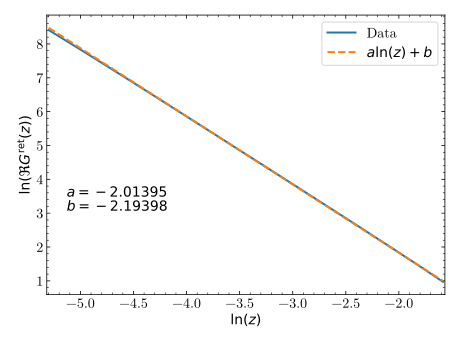
\includegraphics[width=0.48\textwidth]{plots/phase_peak.pdf}
    \caption{Phase Green's function}
\end{figure}

\begin{figure}
    \centering
    \includegraphics[width=0.48\textwidth]{plots/cdw_peak_in_sc.pdf}
    \caption{Log-log plot of the real part of the phase (a) and CDW (b) Green's functions in the SC phase.
        The results for both lattice types are shown but are qualitatively identical.
        The power-law exponent is $a=-2$ and $a=-1$, respectively, indicating that the CDW peak is a $\delta$ distribution, while the phase peak is the derivative of one.}
        \label{fig:peaks_in_sc}
\end{figure}


\textcolor{red}{Die Festellung, dass die Peaks deltas bzw Ableitungen von deltas sind, könnte ich mir auch in einem Anhang vorstellen.}
To further classify the aforementioned peak that lies outside the two-particle continuum,
we turn towards the real part of the Green's function.
We plot it in close proximity to the peaks with a double logarithmic scale and fit the result linearly to obtain its power-law behaviour.
In practice, we use
\begin{align}
    \ln(\Re[\mathcal{G}](\omega - \omega_0 )) &= a \ln(\omega - \omega_0) + b \nonumber \\ 
    \Leftrightarrow \Re[\mathcal{G}] (\omega) &= (\omega - \omega_0)^a e^b\,,
\end{align}
where $\omega_0$ is the peak's position and $a, b$ are fit parameters.
The real part is related to the imaginary part via the Kramers-Kronig relations. \textcolor{red}{Zitiert man die oder nimmt man an, dass jeder weiß, worum es da geht?}
Specifically, if the imaginary part is a $\delta$ distribution, the real part will be proportional to $1/\omega$, i.e., $a=-1$ and the peak has the weight $\exp(b)$.
Furthermore, an exponent of $a=-2$ corresponds to the derivative of the $\delta$ distribution, i.e., $\delta'(\omega - \omega_0)$.

The plots for the phase peak and the CDW peak in the SC phase can be seen in \autoref{fig:peaks_in_sc}.
The SC peak in the CDW phase behaves similarly to the latter and is therefore not shown explicitly.
We get a good agreement with the power-law behaviour near the peaks with the exponents $a=-2$ (phase) and $a=-1$ (CDW), respectively.
Therefore, we conclude that the CDW peak corresponds to a $\delta$ distribution, while the phase peak is its derivative.
Note, that the latter is located at $\omega=0$ of a perfectly asymmetrical bosonic spectral function and therefore must have 0 weight.
This is given here, because $\int \delta'(\omega) \mathrm{d}\omega = 0$.
The peak itself can be interpreted as two $\delta$ distributions at $0^\pm$.

\begin{figure}
    \centering
    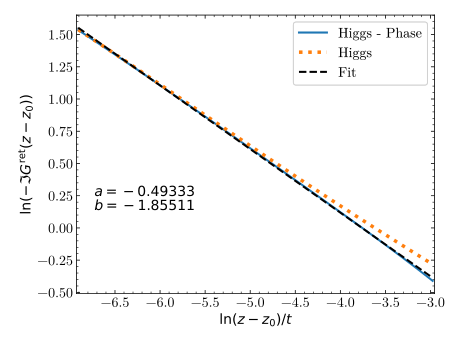
\includegraphics[width=.48\textwidth]{plots/higgs_peak.pdf}
    \caption{Log-log plot of the Higgs spectral function near $\omega = \omega_0 = 2\Delta_\text{SC}$ in the SC phase.
    We additionally plot the difference between the Higgs and the phase spectral functions and fit it, as we interpret the latter as a background within the two-particle continuum.
    The upper (lower) panel shows the results for the square (simple cubic) lattice.
    The spectral function behaves as $1 / \sqrt{\omega - \omega_0}$.}
    \label{fig:higgs_peak}
\end{figure}

Next, we will investigate the Higgs peak. 
Additionally, we see in \autoref{fig:resolvent_overview_SC} that the Higgs and phase spectral functions become indistinguishable towards the upper half of the two-particle continuum.
Therefore, we interpret the latter as a background to the Higgs peak itself and compute the difference between both spectral functions.
We plot the result double logarithmically and fit it again linearly, as seen in \autoref{fig:higgs_peak}.
This time around, the exponent is $a\approx-0.5$, indicating that the peak behaves as $1 / \sqrt{\omega - \omega_0}$.

\begin{figure*}
    \centering
    \includegraphics[width=.98\textwidth]{plots/sc_peak_in_cdw_position.pdf}
    \caption{The upper panels show double logarithmic plots of the positions $\omega_0$ of the SC peak in the CDW phases while the lower panels show their respective weights $w_0 = e^{b}$.
    The left column shows the results for the square and the right column for the simple cubic lattice at $U=-2.5$.
    The fits are linear, i.e., $y(V) = c \ln(V/t) + d$, and the parameters are printed on the individual panels.}
    \label{fig:sc_in_cdw_behaviour}
\end{figure*}

With the prevalent peaks discussed, we turn towards their behaviour as the system approaches the phase transition at $V=0$.
\textcolor{red}{TODO; weiter beschreiben}

\subsection{AFM-CDW transition}

\begin{figure*}
    \centering
    \includegraphics[width=.98\textwidth]{plots/resolvent_overview_AFM_CDW.pdf}
    \caption{Spectral functions with respect to the operators listed in \eqref{eqn:resolvent_bases}.
    The left column shows the results for the square lattice while the right column shows the results for the simple cubic lattice.
    %The left edge of the plots is at $-0.05$ rather than $0$ in order to improve the visibility of the phase peak.
    The shaded area marks the two-particle continuum.
    The panels (a) and (b) show the spectral functions in the CDW and AFM phases, respectively.}
    \label{fig:resolvent_overview_AFM}
\end{figure*}

Similar to the previous section, we will first show the general form of the spectral functions with respect to the operators \eqref{eqn:resolvent_bases}.
They are depicted in \autoref{fig:resolvent_overview_AFM}, choosing $V=1$ for the square lattice and $V=0.75$ for the simple cubic lattice.
For the CDW phase (panel a) we chose $U=zV + 0.1$ and for the AFM phase (panel b) $V=zV - 0.1$.


%%%%%%%%%%%%%%%%%%%%%%%%%%%%%%%%%%%%%%%%%%%%%%%%%%%%%%%%%%%%%%%%%%%%%%%%%%%%%%%%%%%%%%%%%%%%%%%%%%%%%%%%%%%%%%%%%%%%%
%%%%%%%%%%%%%%%%%%%%%%%%%%%%%%%%%%%%%%%%%%%%%%%%%%%%%%%%%%%%%%%%%%%%%%%%%%%%%%%%%%%%%%%%%%%%%%%%%%%%%%%%%%%%%%%%%%%%%
%%%%%                                                Conclusion                                                 %%%%%
%%%%%%%%%%%%%%%%%%%%%%%%%%%%%%%%%%%%%%%%%%%%%%%%%%%%%%%%%%%%%%%%%%%%%%%%%%%%%%%%%%%%%%%%%%%%%%%%%%%%%%%%%%%%%%%%%%%%%
%%%%%%%%%%%%%%%%%%%%%%%%%%%%%%%%%%%%%%%%%%%%%%%%%%%%%%%%%%%%%%%%%%%%%%%%%%%%%%%%%%%%%%%%%%%%%%%%%%%%%%%%%%%%%%%%%%%%%

\section{Conclusion}\label{sec:conclusion}

...

%==============================================================================
% Acknowledgments 
%==============================================================================
\begin{acknowledgments} 
    ....
\end{acknowledgments}

\appendix
\section{Obtaining Green's functions from the iEoM-matrices}



Nevertheless, let us show that $\mathcal{M}$ is positive semidefinite if the system is in thermal equilibrium.
For any $\vec{x} \in \mathbb{C}^N$, consider
\begin{align}
    \vec{x}^\dagger \mM \vec{x} &= \sum_{ij} x_i^* x_j \mM_{ij} \nonumber \\
        &= \langle \left[ \sum_i x_i^* A_i^\dagger, \left[ H, \sum_j x_j A_j \right] \right]  \rangle \nonumber \\
        &= \langle [B^\dagger, [H, B]] \rangle\,,\quad B \coloneqq  \sum_j x_j A_j\,.
\end{align}
Expanding the thermal expectation value $\langle O \rangle = \frac{1}{Z} \Trace [\exp(-\beta H_\text{MF}) O]$, where $\beta$ is the inverse temperature and $Z$ the partition function, and the commutators, we obtain

\begin{widetext}
    \begin{align}
        \langle [B^\dagger, [H, B]] \rangle &= \frac{1}{Z} \Trace [\exp(-\beta H) [B^\dagger, [H, B]]] \nonumber \\
            &= \frac{1}{Z} \sum_j e^{-\beta \epsilon_j} \bra{\psi_j} [B^\dagger, [H, B]] \ket{\psi_j} \nonumber \\
            &= \frac{1}{Z} \sum_j e^{-\beta \epsilon_j} \left[ \bra{\psi_j} B^\dagger (H - \epsilon_j) B \ket{\psi_j} + \bra{\psi_j} B (H - \epsilon_j) B^\dagger \ket{\psi_j} \right] \nonumber \\
            &= \frac{1}{Z} \sum_{ij} e^{-\beta \epsilon_j} \left[ \bra{\psi_j} B^\dagger \ket{\psi_i} (\epsilon_i - \epsilon_j) \bra{\psi_i} B \ket{\psi_j} + \bra{\psi_j} B \ket{\psi_i} (\epsilon_i - \epsilon_j) \bra{\psi_i} B^\dagger \ket{\psi_j} \right] \nonumber \\
            &= \frac{1}{Z} \sum_{ij} e^{-\beta \epsilon_j} (\epsilon_i - \epsilon_j) \underbrace{ \left[ \bra{\psi_j} B^\dagger \ket{\psi_i} \bra{\psi_i} B \ket{\psi_j} + \bra{\psi_j} B \ket{\psi_i} \bra{\psi_i} B^\dagger \ket{\psi_j} \right]}_{\coloneqq C_{ij} = C_{ji} \geq 0} \nonumber \\
            &= \frac{1}{2Z} \left[ \sum_{ij} C_{ij} e^{-\beta \epsilon_j} (\epsilon_i - \epsilon_j) - \sum_{ij} C_{ij} e^{-\beta \epsilon_i} (\epsilon_i - \epsilon_j) \right] \nonumber \\
            &= \frac{1}{2Z} \sum_{ij} C_{ij} \left( e^{-\beta \epsilon_j} - e^{-\beta \epsilon_i} \right) \left( \epsilon_i - \epsilon_j \right) \geq 0\,.
    \end{align}
\end{widetext}

Thus, we are able to compute a real square root of $\mathcal{M}$.

\bibliography{sn-bibliography}
%\bibliography{../../A_bibinput/liter10.bib}
		
\end{document}
